\documentclass[fontsize=12pt]{scrartcl}

\newcommand{\grad}{\ensuremath{^{\circ}} }
\renewcommand{\strut}{\vrule width 0pt height5mm depth2mm}

\usepackage[utf8]{inputenc}
\usepackage[final]{pdfpages}
% obere Seitenränder gestalten können
\usepackage{fancyhdr}
\usepackage{moreverb}
% Graphiken als jpg, png etc. einbinden können
\usepackage{graphicx}
%\usepackage{stmaryrd}
% Floats Objekte mit [H] festsetzen
\usepackage{float}
% setzt URLs schön mit \url{http://bla.laber.com/~mypage}
\usepackage{url}
% Externe PDF's einbinden können
\usepackage{pdflscape}
% Verweise innerhalb des Dokuments schick mit " ... auf Seite ... "
% automatisch versehen. Dazu \vref{labelname} benutzen
\usepackage[ngerman]{varioref}
\usepackage[ngerman]{babel}
\usepackage{ngerman}
% Bibliographie
\usepackage{bibgerm}
% Tabellen
\usepackage{tabularx}
\usepackage{supertabular}
\usepackage[colorlinks=true, pdfstartview=FitV, linkcolor=blue,
            citecolor=blue, urlcolor=blue, hyperfigures=true,
            pdftex=true]{hyperref}
\usepackage{bookmark}
\usepackage[a4paper, twoside]{geometry}

% Damit Latex nicht zu lange Zeilen produziert:
\sloppy
%Uneinheitlicher unterer Seitenrand:
%\raggedbottom

% Kein Erstzeileneinzug beim Absatzanfang
% Sieht aber nur gut aus, wenn man zwischen Absätzen viel Platz einbaut
\setlength{\parindent}{0ex}

% Abstand zwischen zwei Absätzen
\setlength{\parskip}{1ex}

\addtolength{\evensidemargin}{-2cm}
\addtolength{\oddsidemargin}{2cm}

% Lustige Header auf den Seiten
  \pagestyle{fancy}
 \setlength{\headheight}{70.55003pt}
  \fancyhead{}
  \fancyhead[LO,RE]{Benutzerhandbuch}
  \fancyhead[LE,RO]{Seite \thepage\\\slshape \leftmark\\\slshape \rightmark}

%
% Und jetzt geht das Dokument los....
%

\begin{document}

% Start Titelseite
  \thispagestyle{empty}
  \newgeometry{hmarginratio=1:1}
  \vspace{3cm}
  \begin{minipage}[H]{\textwidth}
  \begin{center}
  \vspace{1cm}
  \bf
  {\Large Benutzerhandbuch}\\
  der Stundenplansoftware \\
  der Gruppe\\
    \begin{figure}[H]
    \centering
    
\includegraphics[width=0.15\textwidth]{../WOYM.png}
    \end{figure}
  \vfill
  \end{center}
  \end{minipage}
  \vfill
  \begin{minipage}[H]{\textwidth}
  \begin{center}
  \sf
  \begin{tabular}{l}
  Tim Hansen \\\
  Adrian Lück \\
  Jurij Schmidt\\
  \end{tabular}
  \end{center}
  \end{minipage}
\restoregeometry
% Ende Titelseit

% Start Leerseite
\cleardoubleemptypage

%Start Inhaltsverzeichnis
\newpage

  \thispagestyle{fancy}
  \fancyhead{}
  \fancyhead[LO,RE]{Benutzerhandbuch}
  \fancyhead[LE,RO]{Seite \thepage\\\slshape \leftmark~}
  \fancyfoot{}
  \renewcommand{\headrulewidth}{0.4pt}
  \tableofcontents

\newpage
  \fancyhead[LE,RO]	{Seite \thepage\\ \slshape \leftmark \\ \slshape \rightmark}

\section{Systemanforderungen}
\begin{itemize}
\item Java 7 oder neuer
\item ein aktueller Webbrowser
\end{itemize}

\section{Installation und Inbetriebnahme}

Entpacken Sie die ausgelieferte ZIP-Datei in das von Ihnen für die Software gewünschte Arbeitsverzeichnis. 

\subsection{Windows-Betriebssysteme}
Unter Windows können Sie die Datei \textit{start.bat} verwenden, um die Software zu starten. Wenn Sie die Datei anklicken öffnet sich die Windows-Konsole und der für die Software benötigte Server startet. Gleichzeitig öffnet sich Ihr Browser-Fenster und lädt die Startseite der Software, sobald der Server komplett hochgefahren ist. Schließen Sie die Windows-Konsole nur, wenn Sie die Software beenden wollen. Ansonsten muss Sie für den Betrieb der Software geöffnet bleiben.\\
Wenn Sie wünschen, die Software vom Desktop aus starten zu können, legen Sie eine Verknüpfung zu der Datei \textit{start.bat} an.

\subsection{Linux- / Mac-Betriebssysteme}

\section{Bedienung der Software}

\subsection{Allgemeine Informationen}

Sie können nahezu alle Aktionen, die sie ausgeführt haben rückgängig machen oder das Rückgängigmachen wiederholen. Die einzige Ausnahme bildet das Ändern der Systemeinstellungen. Dies lässt sich nur manuell rückgängig machen und alle Aktivitäten, die dabei möglicherweise gelöscht wurden, lassen sich nicht wiederherstellen ohne ein Backup eines vorherigen Zeitpunktes zu laden.\\

Die Software ist grundsätzlich in zwei Seiten, die Einrichtungs- und die Planungsseite eingeteilt. Auf beiden Seiten werden Sie oben eine angepinnte Toolbar finden, welche Ihnen das Rückgängigmachen und Wiederherstellen von bis zu zehn Aktionen und das Wechseln auf die jeweils andere Seite erlaubt. Beispielhaft ist hier die Toolbar der Einrichtungsseite dargestellt.

\begin{figure}[H]
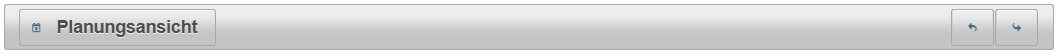
\includegraphics[width=\textwidth]{images/bar.png}
\caption{Toolbar der Einstellungsseite}
\end{figure}

\subsection{Die Einrichtungsseite}
Die Einrichtungsseite dient der Vorbereitung zur Planung. Sie legen dort Standorte und Räume, Unterrichtsinhalte, Schulklassen, Personen des Personals und Klassenteams an und verwalten ihre Systemeinstellungen und Backups. Es wird empfohlen zunächst die Systemeinstellungen an Ihre Bedürfnisse anzupassen und anschließend die Objekte nach der Reihenfolge des Navigationsmenüs von oben nach unten hinzuzufügen.
\begin{figure}[H]
\centering
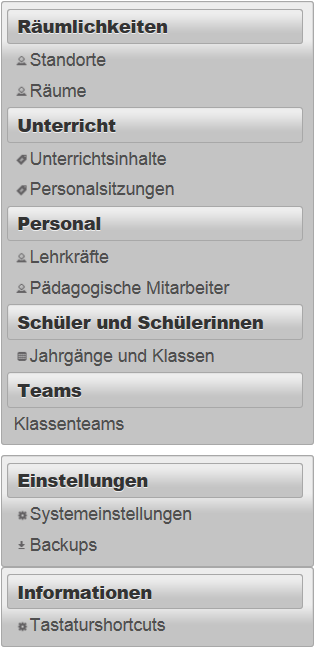
\includegraphics[width=0.3\textwidth]{images/navigationMenu.png}
\caption{Navigationsmenü auf der Einstellungsseite}
\end{figure}

Da für das Hinzufügen, Bearbeiten und Löschen aller Objekte dieselbe Mechanik verwendet wird, wird dies im Folgenden lediglich am Beispiel einer Lehrkraft erläutert.

\subsubsection{Systemeinstellungen}
In den Systemeinstellungen können Sie verschiedene Parameter der Software selbst festlegen.\\

Zunächst einmal haben Sie in den Systemeinstellungen die Möglichkeit, alle Aktivitäten zu löschen, falls Sie eine komplett neue Planung beginnen möchten. Diesen Schritt können Sie rückgängig machen. 

\begin{figure}[H]
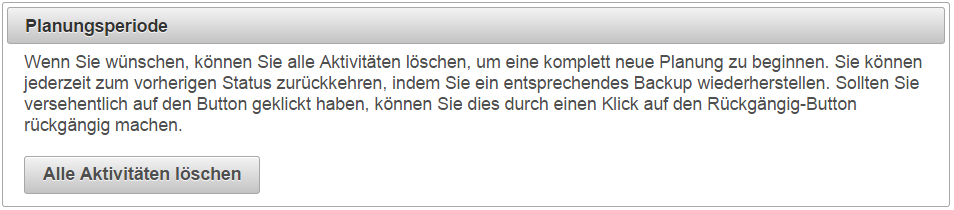
\includegraphics[width=\textwidth]{images/systemSettings1.png}
\caption{Einstellungsseite: Alle Aktivitäten löschen}
\end{figure}

Des Weiteren können Sie die allgemeinen Einstellungen der Software verändern. So haben Sie etwa die Möglichkeit die zu verplanenden Wochentage, Start- und Endzeit eines Wochentags und die Größe des Zeitrasters des Stundenplans festzulegen. Außerdem können Sie angeben, wie die zeitliche Abrechnung des Personals erfolgen soll, welche Bezeichner sie für Schulklassen wünschen und wie lang die typische Dauer einer Aktivität sein soll. Sie können hier außerdem alle Dialoge zurücksetzen, so dass diese erneut beim Löschen angezeigt werden. \\

\fbox{\parbox{\textwidth}{\textbf{Achtung!} Wenn Sie die zu verplanenden Wochentage oder die Start- und Endzeit eines Wochentages ändern, werden alle Aktivitäten gelöscht, die an nicht mehr gewählten Wochentagen und außerhalb der neuen Start- und Endzeit liegen. Dies lässt sich \textbf{nicht} über den Rückgängig-Button rückgängig machen. Stattdessen müssten Sie ein Backup eines Zeitpunktes laden, wo sich die Aktivitäten noch im System befinden.}}

\begin{figure}[H]
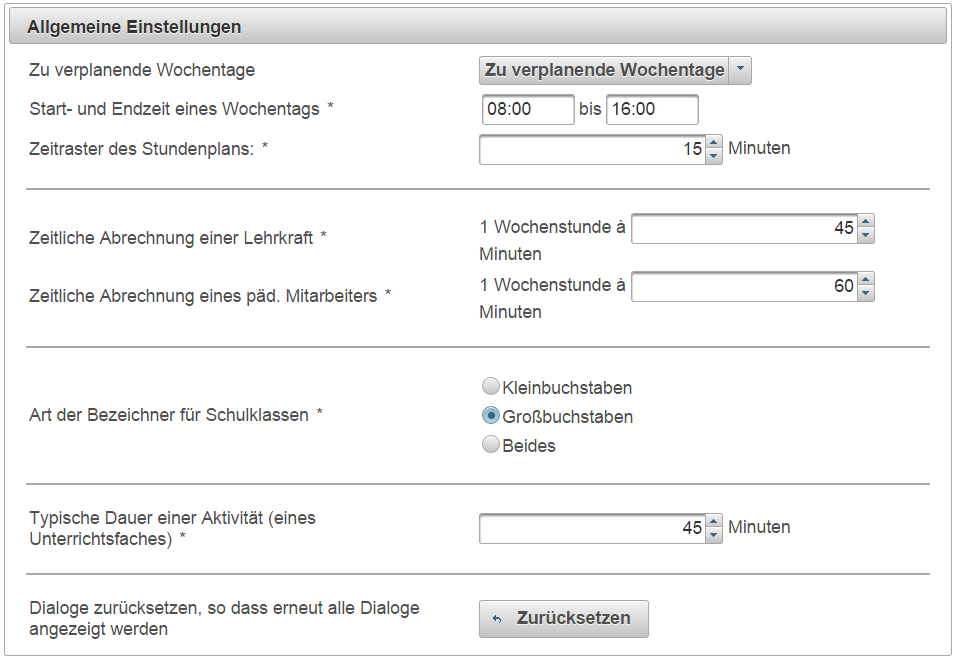
\includegraphics[width=\textwidth]{images/systemSettings2.png}
\caption{Allgemeine Einstellungen}
\end{figure}


Schließlich können Sie auf der Einstellungsseite auch noch das Intervall für automatische Backups festlegen. Hier können Sie wählen, dass Sie keine automatischen Backups, Backups in einem gewissen Minutentakt oder Backups in einem gewissen Tagestakt zu einer bestimmten Uhrzeit wünschen. Wenn Sie letztere Option wählen und die Software zu dem eigentlichen Backup-Zeitpunkt nicht gestartet ist, wird beim nächsten Programmstart nachträglich ein Backup ausgeführt.

\fbox{\parbox{\textwidth}{\textbf{Achtung!} Beachten Sie, dass Backups nicht automatisch gelöscht werden! Für weitere Informationen bezüglich der Backups, lesen Sie das folgende Kapitel.}}
 
\begin{figure}[H]
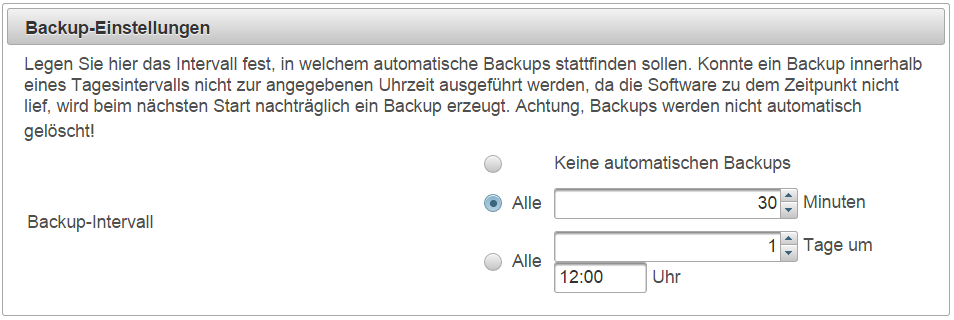
\includegraphics[width=\textwidth]{images/systemSettings3.png}
\caption{Backup-Einstellungen}
\end{figure}

\subsubsection{Anlegen und Wiederherstellen von Backups}

In dieser Software entspricht ein Backup im Grunde einem Speicherstand des System zu einem gewissen Zeitpunkt. In einem Backup ist nicht nur der Datenbankzustand, sondern auch die Systemeinstellungen des Zeitpunktes, an welchem das Backup erstellt wurde, vorhanden. Wie aus dem vorherigen Kapitel hervorging, ist die Software in der Lage Backups automatisch im Hintergrund zu erzeugen. Zusätzlich oder wenn Sie die automatischen Backups ausgeschaltet haben, können Sie aber auch manuell Backups erzeugen. \\
Sie haben die Auswahl, ob ein Backup einen automatisch aus dem aktuellen Datum und der Uhrzeit generierten Namen tragen soll oder ob sie es selbst benennen möchten.\\
Die Backups werden in Ihrem Benutzer-Ordner, wo sich auch der aktuelle genutzte Datenbankzustand befindet, gespeichert. Unter Windows ist der Pfad zum Backup-Ordner \textit{C:\textbackslash{}Users\textbackslash{}Username\textbackslash{}WOYM} unter Linux/Mac-OS \textit{/home/username/WOYM}. Dort werden die Backups als ZIP-Dateien abgelegt.\\
Die Backups werden auf der Backupverwaltung-Seite absteigend nach Erstellungsdatum sortiert.

\begin{figure}[H]
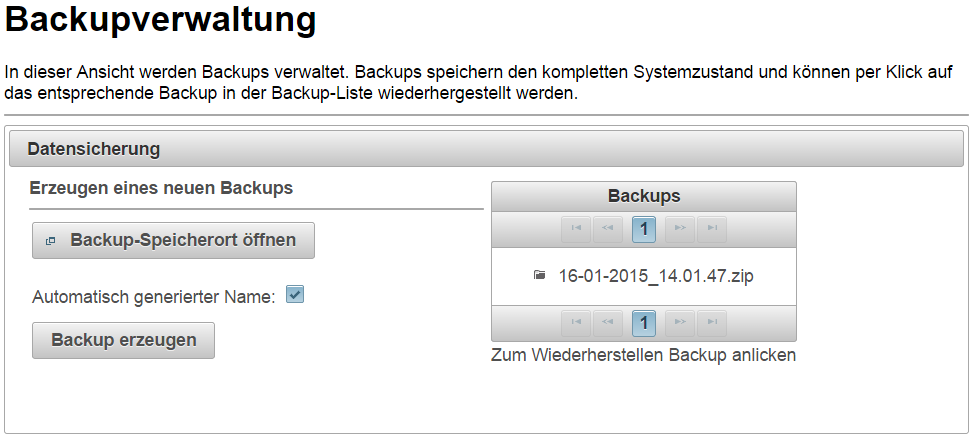
\includegraphics[width=\textwidth]{images/backupManagement.png}
\caption{Backupverwaltung}
\end{figure}

\subsubsection{Hinzufügen eines Objektes am Beispiel einer Lehrkraft}
\begin{enumerate}
\item Klicken Sie im Menü auf der linken Seite auf den Eintrag "`Lehrkräfte"'.
\item Sie sehen nun eine Tabelle, in welcher alle vorhandenen Lehrkräfte angezeigt werden. Klicken Sie auf den "`Hinzufügen"'-Button oben rechts.
\item Das folgende Dialogfenster öffnet sich: \medskip\\
	\begin{minipage}[t]{\linewidth}
            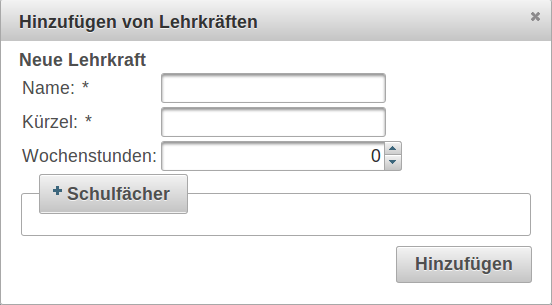
\includegraphics[width=.8\linewidth]{images/addTeacherDialog.png}
    \medskip\\
    Die mit * gekennzeichneten Angaben sind Pflichtangaben. Der Eintrag "`Schulfächer"' ist aufklappbar. Aufklappbare Angaben sind immer optional.
    \end{minipage}
\clearpage
\item Machen Sie alle gewünschten Angaben und klicken Sie anschließend auf "`Hinzufügen"'. Sie werden darüber informiert, wenn das Hinzufügen erfolgreich war: \medskip\\
	\begin{minipage}[t]{\linewidth}
            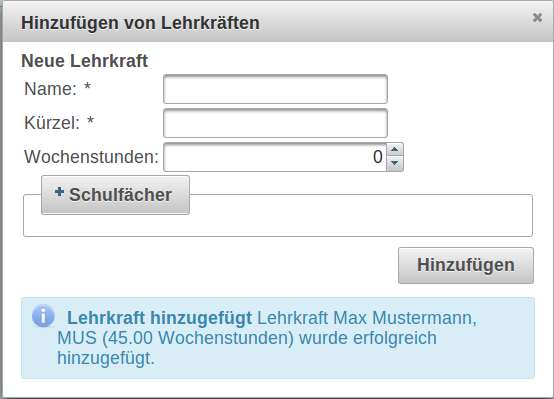
\includegraphics[width=.8\linewidth]{images/addedTeacher.png}
    \medskip\\
    Das Dialogfenster bleibt geöffnet, um das Hinzufügen weiterer Lehrkräfte zu erlauben. Wenn Sie keine weitere Lehrkraft hinzufügen möchten, klicken Sie auf das X in der oberen rechten Ecke des Dialogs.
    \end{minipage}
\end{enumerate}

\subsubsection{Aktualisieren eines Objektes am Beispiel einer Lehrkraft}

\begin{enumerate}
\item Führen Sie einen Rechtsklick auf die zu bearbeitende Lehrkraft aus und wählen sie "`Bearbeiten"': \medskip\\
	\begin{minipage}[t]{\linewidth}
            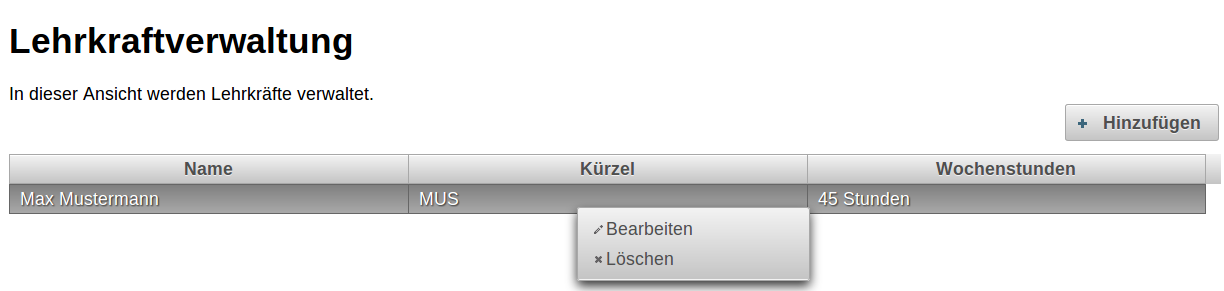
\includegraphics[width=1\linewidth]{images/editTeacher.png}
    \end{minipage}
\item Im dem sich öffnenden Dialogfenster sind alle Angaben der gewählten Lehrkraft eingetragen: \medskip\\
	\begin{minipage}[t]{\linewidth}
            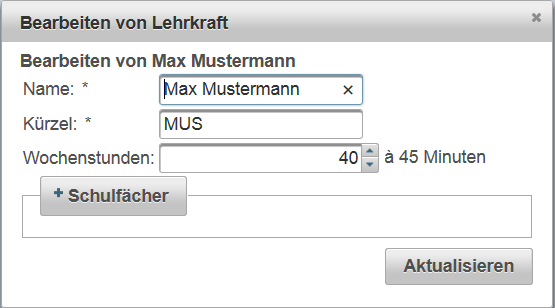
\includegraphics[width=.8\linewidth]{images/editTeacherDialog.png}
    \medskip\\ Passen Sie die Angaben nach Belieben an.
    \end{minipage}
\item Klicken Sie auf "`Aktualisieren"'. Bei Erfolg schließt sich das Dialogfenster und Sie werden über die erfolgreiche Aktualisierung informiert. 
\end{enumerate}

\subsubsection{Löschen eines Objektes am Beispiel einer Lehrkraft}
\begin{enumerate}
\item Führen Sie einen Rechtsklick auf die zu bearbeitende Lehrkraft aus und wählen sie "`Löschen"': \medskip\\
	\begin{minipage}[t]{\linewidth}
            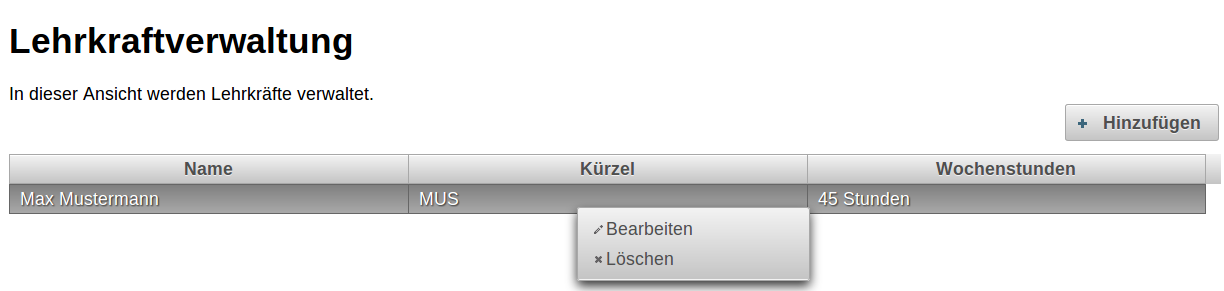
\includegraphics[width=1\linewidth]{images/editTeacher.png}
    \end{minipage}
\item Es öffnet sich ein Dialogfenster, welches Sie über die Folgen des Löschens aufklärt. Da Sie alle Aktionen rückgängig machen können, haben Sie die Option, das Dialogfenster zukünftig nicht mehr anzeigen zu lassen. \medskip\\
	\begin{minipage}[t]{\linewidth}
            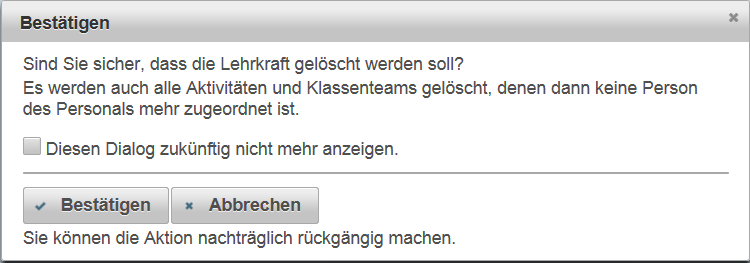
\includegraphics[width=.8\linewidth]{images/confirmDialog.png}
    \end{minipage} 
\end{enumerate}

\section{Planungsseite}

\section{Fehler und Fehlerbehandlung}

\end{document}
